\Subsection{Queue \& Deque}

\begin{problem}\textbf{Maximum of Sliding Window}

    Given an array of integers $a$, there is a sliding window of size $k$ which is moving from the very left of the array to the very right. You can only see the $k$ numbers in the window. Each time the sliding window moves right by one position.

    Return the array that contains maximum elements of each position of the sliding window.

    Time complexity: $O(n)$.

    Space complexity: $O(k)$.\newline

    \underline{Note}: you can solve it on \href{https://leetcode.com/problems/sliding-window-maximum/description/}{LeetCode}

    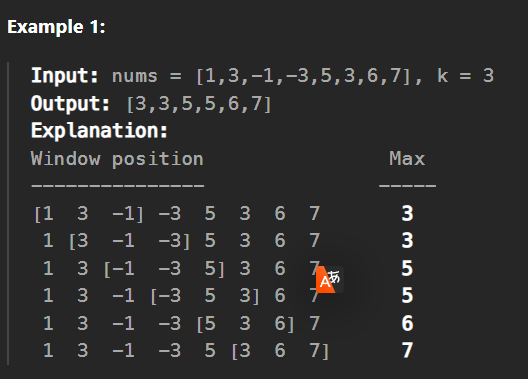
\includegraphics[scale=0.6]{./assets/05-basic-data-structures/1-1.PNG}

    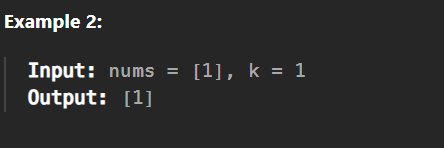
\includegraphics[scale=0.6]{./assets/05-basic-data-structures/1-2.PNG}

\end{problem}


\begin{solution}
    \textbf{\textnumero 1, Using deque + two pointers}

    Credits to \textbf{monster0Freason} for a great \href{https://leetcode.com/problems/sliding-window-maximum/solutions/4628595/19-1-approach-1-o-n-python-c-step-by-step-explanation/}{solution}.

    Let's look at the following example where we see $4$ elements and the window size is $k=3$:

    $a_0=1, a_1=3, a_2=-1, a_3=2$ - for any sliding windows that contain both $a_0$ and $a_1$ can never have $a_0$ as a maximum; same for the sliding windows that contain $a_2$ and either $a_1$ or $a_3$ since $a_2 < a_1, a_3$ $\implies$ we do not care about the elements that are smaller than those we currently capture in a sliding window of size $k$.

    Let's then capture only elements such that $a_{i_1} \geq a_{i_2} \geq ... \geq a_{i_{\bar{k}}} (\bar{k} \leq k)$. Then for the current sliding window the result is $a_{i_1}$ since it is the greatest element among those captured by this sliding window. In order to move the sliding window to the next element we need to consider the next element $a_r$ and remove all $a_{i_j}..a_{i_{\bar{k}}} < a_r$ to preserve the defined above property. In order to support such an algorithm we could use \textbf{deque}:


    \begin{lstlisting}[language=C++]
    void solve(const std::vector<int>& a, int k) {
        // keeping indexes because it eases the removal of the leftmost element
        // once it gets out of the sliding window range.
        std::deque<int> d;

        int left = 0;
        int right = 0;

        while (right < a.size()) {
            while(!d.empty() && a[d.back()] < a[right]) {
                d.pop_back();
            }
            d.push_back(right);
            // now we preserve the invariant: a[d[0]] >= a[d[1]] >= a[d[2]] ...

            if (left > d.front()) {
                d.pop_front();
            }

            // once we have observed enough elements for the 1st sliding window
            if (right >= k - 1) {
                std::cout << a[d.front()] << " ";
                left++;
            }
            right++;
        }
    }
    \end{lstlisting}


    \textbf{\textnumero 2, Using std::multiset + two pointers}

    We have not yet studied sets and multisets (i.e. \textbf{std::set<T>} and \textbf{std::multiset<T>}) but it is also a possible solution which works in $O(n \cdot \log{k})$ of time complexity.

    In C++ \textbf{std::set} and \textbf{std::multiset} are the data structures that keep the sorted set of the elements witout or with duplicates respectively. By default both of them sort elements in ascending order but it is possible to sort in the descending order as well (\textbf{std::multiset<T, std::greater<T> >}, e.g., for int: \textbf{std::multiset<int, std::greater<int> >} (same for \textbf{std::set<T>}); see template parameters of the structures on \href{https://cppreference.com}{cppreference.com}). In order to retrieve the maximum element in the set we need to call its \textbf{begin()} method which returns an iterator to the beginning (\textbf{works for $O(\log{(size)})$!}):

    \begin{lstlisting}[language=C++]
    std::set<int, std::greater<int>> s1;
    s1.insert(2);
    s1.insert(1);
    s1.insert(3);
    // (*s1.begin()) == 3; s1 = {3, 2, 1}

    std::set<int> s2;
    s2.insert(2);
    s2.insert(1);
    s2.insert(3);
    // (*s2.begin()) == 1; s2 = {1, 2, 3}
    \end{lstlisting}

    Here we keep a sliding window of size $k$ by both \textbf{left} and \textbf{right} pointers and add the next element under \textbf{right} and remove an element under \textbf{left} once we shift the sliding window. After shifting the sliding window we retrieve the maximum and print it:

    \begin{lstlisting}[language=C++]
    void solve(const std::vector<int>& a, int k) {
        std::multiset<int, std::greater<int>> st;
        int left = 0;
        int right = 0;

        for (; right < std::min(a.size(), k); ++right) {
            st.insert(a[right]);
        }

        std::cout << (*st.begin()) << " ";

        while(right < a.size()) {
            // removing via iterator, but the element.
            // st.erase(val) would remove all elements that are equal to 'val'
            st.erase(st.find(a[left++]));
            st.add(a[right++]);
            std::cout << (*st.begin()) << " ";
        }
    }
    \end{lstlisting}

\end{solution}





\begin{problem}\textbf{Max Value of Equation}

    Given an array $p$ of size $n \leq 10^5$ containing the coordinates of points on a 2D plane, sorted by the $x$-values, i.e. $\{ x_i \}$ form a strictly increasing sequence ($x_i < x_j, \ i < j$), where $p_i = (x_i, y_i)$ ($-10^8 \leq x_i, y_i \leq 10^8$). You are also given an integer $k \leq 2\cdot 10^8$.

    Return the \textbf{maximum value of the equation} $y_i + y_j + |x_i - x_j|$ where $|x_i - x_j| \leq k$ and $0 \leq i < j < n$.

    It is guaranteed that there exists at least one pair of points that satisfy the constraint $|x_i - x_j| \leq k$.

    Time complexity: $O(n)$ or $O(n \cdot \log{n})$.

    Space complexity: $O(k)$.\newline

    \underline{Note}: you can solve it on \href{https://leetcode.com/problems/max-value-of-equation/description/}{LeetCode}

    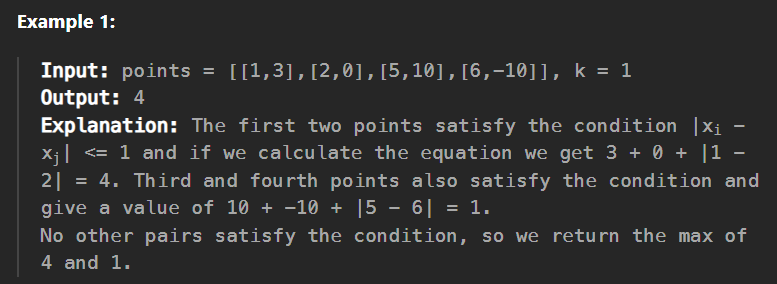
\includegraphics[scale=0.6]{./assets/05-basic-data-structures/2-1.PNG}

    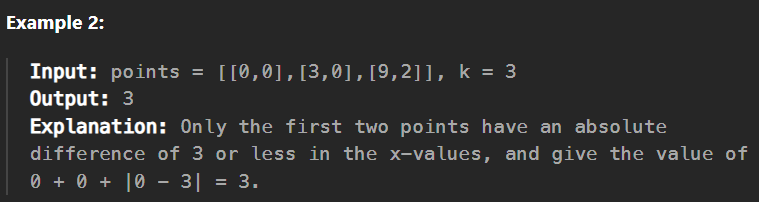
\includegraphics[scale=0.6]{./assets/05-basic-data-structures/2-2.PNG}

\end{problem}


\begin{solution}

    Notice that the points are sorted in ascending order by their $x$-coordinates, thus we can keep a sliding window $(p_{i_1}, p_{i_2}, ..., p_{i_j}), \forall m=1..j: \ p_{i_m} = (x_{i_m}, y_{i_m})$ that satisfies $x_{i_n} \leq x_{i_m}, \ n < m$ and $|x_{i_1} - x_{i_j}| \leq k$, by keeping such a sliding window we automatically satisfy the condition $|x_i - x_j| \leq k$.

    Now let's work with the given formula:

    $y_i + y_j + |x_i - x_j|$ - assume that $i < j$ $\implies$ $(y_i-x_i) + (y_j+x_j)$. Since the answer always exists, therefore, such $j$ exists either $\implies$ let's assume that every time when we add a next point $p = (x, y)$ into own sliding window, this added point $p$ substitutes its coordinate components $x, y$ in the formula as $x_j, y_j$, i.e. $x_j := x$ and $y_j := y$.

    Notice that now we only have $y_i-x_i$ as unfixed part of the sum, thus we need to maximize it $\implies$ we need to find such a point $\bar{p}_i$ whose $y_i-x_i \to \max$; we already know that this $p$ is contained in our sliding window by definition $\implies$ we need to find maximum in the sliding window over the function $y_i-x_i$, we can easily do it via \textbf{max-queue} over pairs \textbf{($y_i-x_i$, $x_i$)} where maximum is built over 1st component of the pair:

    \begin{lstlisting}[language=C++]
    void solve(const std::vector<pair<int, int>>& points, int k) {
        MaxQueue<pair<int, int>> q;
        int ans = INT_MIN;

        for (int i = 0; i < points.size(); ++i) {
            while(!q.empty() && std::abs(q.front().second - points[i].x) > k
                /* <=> |xi - xj| > k */) {
                q.pop_front();
            }
            // before adding current point we relax the answer

            // q.retrieveMax() returns a pair {yi-xi, xi}
            // see: structured binding in C++
            auto [diff, x] = q.retrieveMax();

            ans = std::max(ans, diff + points[i].y + points[i].x);
            q.push_back({ points[i].y - points[i].x, points[i].x });
        }

        std::cout << ans << std::endl;
    }
    \end{lstlisting}



\end{solution}